\documentclass{beamer}\usepackage[]{graphicx}\usepackage[]{xcolor}
% maxwidth is the original width if it is less than linewidth
% otherwise use linewidth (to make sure the graphics do not exceed the margin)
\makeatletter
\def\maxwidth{ %
  \ifdim\Gin@nat@width>\linewidth
    \linewidth
  \else
    \Gin@nat@width
  \fi
}
\makeatother

\definecolor{fgcolor}{rgb}{0.345, 0.345, 0.345}
\newcommand{\hlnum}[1]{\textcolor[rgb]{0.686,0.059,0.569}{#1}}%
\newcommand{\hlstr}[1]{\textcolor[rgb]{0.192,0.494,0.8}{#1}}%
\newcommand{\hlcom}[1]{\textcolor[rgb]{0.678,0.584,0.686}{\textit{#1}}}%
\newcommand{\hlopt}[1]{\textcolor[rgb]{0,0,0}{#1}}%
\newcommand{\hlstd}[1]{\textcolor[rgb]{0.345,0.345,0.345}{#1}}%
\newcommand{\hlkwa}[1]{\textcolor[rgb]{0.161,0.373,0.58}{\textbf{#1}}}%
\newcommand{\hlkwb}[1]{\textcolor[rgb]{0.69,0.353,0.396}{#1}}%
\newcommand{\hlkwc}[1]{\textcolor[rgb]{0.333,0.667,0.333}{#1}}%
\newcommand{\hlkwd}[1]{\textcolor[rgb]{0.737,0.353,0.396}{\textbf{#1}}}%
\let\hlipl\hlkwb

\usepackage{framed}
\makeatletter
\newenvironment{kframe}{%
 \def\at@end@of@kframe{}%
 \ifinner\ifhmode%
  \def\at@end@of@kframe{\end{minipage}}%
  \begin{minipage}{\columnwidth}%
 \fi\fi%
 \def\FrameCommand##1{\hskip\@totalleftmargin \hskip-\fboxsep
 \colorbox{shadecolor}{##1}\hskip-\fboxsep
     % There is no \\@totalrightmargin, so:
     \hskip-\linewidth \hskip-\@totalleftmargin \hskip\columnwidth}%
 \MakeFramed {\advance\hsize-\width
   \@totalleftmargin\z@ \linewidth\hsize
   \@setminipage}}%
 {\par\unskip\endMakeFramed%
 \at@end@of@kframe}
\makeatother

\definecolor{shadecolor}{rgb}{.97, .97, .97}
\definecolor{messagecolor}{rgb}{0, 0, 0}
\definecolor{warningcolor}{rgb}{1, 0, 1}
\definecolor{errorcolor}{rgb}{1, 0, 0}
\newenvironment{knitrout}{}{} % an empty environment to be redefined in TeX

\usepackage{alltt}

\usepackage{graphicx}
\usepackage{lscape}
\usepackage{changepage}
%\usepackage{graphicx}
\usepackage{etoolbox}
\usepackage{everysel}
\usepackage{textcomp}

%% This sets the theme of the presentation which controls
%% the formatting of the slides
\usetheme{Boadilla}

%% Turn off the navigation symbols
\setbeamertemplate{navigation symbols}{} 


%% Set the author block so STATS 201/8 appears on every
\author{STATS 201/8}

%% Clear the date block
\date{}


%% This makes all equations blue
\AtBeginEnvironment{equation*}{\color{blue}}
\AtBeginEnvironment{align*}{\color{blue}}
\everymath{\color{blue}}

%% This puts a 6 point space between paragraphs, means we don't need to use vspace, or list environments if 
%% we don't want to
\setlength{\parskip}{0pt}


%% Russell: removes spaces after R input/output?
%% \setlength{\topsep}{0mm}

%% Some useful colors
\definecolor{darkgreen}{rgb}{0.176,0.486,0.031}
\definecolor{redbrown}{HTML}{950605}
\definecolor{darkred}{HTML}{d80605}


%% nice little macro for changing the font of R code
\newcommand{\rcode}[1]{{\color{darkgreen}\texttt{#1}}}

%% macro for bold blue italics
\newcommand{\blueBoldEmph}[1]{{\color{blue}\textbf{\emph{#1}}}}

% ~iid macro
\newcommand{\iid }{\stackrel{iid}{\sim}}
\usepackage{graphicx}
\usepackage{verbatim}
\usepackage{etoolbox}
\usepackage{everysel}
% \usepackage{enumitem}

%% This package allows text highlighting
\usepackage{soul}

%% This sets the theme of the presentation which controls
%% the formatting of the slides
\usetheme{Boadilla}

%% Turn off the navigation symbols
\setbeamertemplate{navigation symbols}{} 

%% Change the default itemize [ball]s to [circle]s
\setbeamertemplate{itemize items}[circle]

%% Change the default enumerate [ball]s to plain text
\setbeamertemplate{enumerate items}[default]

%% Load the enumitem package and ensure it works nicely with beamer
% \setitemize{label=\usebeamerfont*{itemize item}
%   \usebeamercolor[fg]{itemize item}
%   \usebeamertemplate{itemize item}}
% \setenumerate{label=\usebeamerfont*{enumerate item}
%   \usebeamercolor[fg]{enumerate item}
%   \usebeamertemplate{enumerate item}}

%% Set the author block so STATS 201/8 appears on every
\author{STATS 201/8}

%% Clear the date block
\date{}


\setbeamercolor{title}{bg=blue!40}
\setbeamerfont{title}{size=\LARGE,series=\bfseries}

%%Sectioning commands
\setbeamercolor{section title}{bg=blue!20}
\setbeamerfont{section title}{size=\large}

\setbeamertemplate{section page}{%
    \begingroup
        \begin{beamercolorbox}[sep=10pt,center,rounded=true,shadow=true]{section title}
        \usebeamerfont{section title}Section~\thechapter.\thesection \newline \insertsection\par
        \end{beamercolorbox}
		\vfill
    \endgroup
}

\newcommand{\BeginSection}[1]{\section{#1} \frame{\sectionpage}}
%\AtBeginSection[]{%
%    \begin{frame}
%        \sectionpage
%    \end{frame}
%}


%% This makes all equations blue
\AtBeginEnvironment{equation*}{\color{blue}}
\AtBeginEnvironment{align*}{\color{blue}}
\everymath{\color{blue}}

%% This puts a 0 point space between paragraphs, means we don't need to use vspace, or list environments if 
%% we don't want to
\setlength{\parskip}{0pt}


%% Russell: removes spaces after R input/output?
\setlength{\topsep}{0.5mm}

%% David: In addition to Russel's command to remove spaces after R input/output, these commands remove the space between R input/output.
%% Stackoverflow link: https://stackoverflow.com/questions/35734525/reduce-space-between-code-chunks-and-code-output-in-rmarkdown-beamer-presentatio
%% \setlength{\OuterFrameSep}{-2pt}
\makeatletter
\preto{\@verbatim}{\topsep=-1pt \partopsep=-1pt }
\makeatother

%% Some useful colors
\definecolor{darkgreen}{rgb}{0.176,0.486,0.031}
\definecolor{redbrown}{HTML}{950605}
\definecolor{darkred}{HTML}{d80605}


%% nice little macro for changing the font of R code
\newcommand{\rcode}[1]{\protect{\color{darkgreen}\texttt{#1}}}

%% macro for bold blue italics
\newcommand{\blueBoldEmph}[1]{{\color{blue}\textbf{\emph{#1}}}}

% ~iid macro
\newcommand{\iid }{\stackrel{iid}{\sim}}

%% Macro for t-test amd P-value
\newcommand{\ttest}{\emph{t}-test}
\newcommand{\pval}{\emph{P}-value}

%% Statistics operators 
\DeclareMathOperator{\Bias}{Bias}
\DeclareMathOperator{\Cov}{Cov}
\DeclareMathOperator*{\Cor}{Cor}
\DeclareMathOperator{\E}{E}
\DeclareMathOperator{\MSE}{MSE}
\DeclareMathOperator{\Odds}{Odds}
\DeclareMathOperator{\OR}{OR}
\DeclareMathOperator{\PMSE}{PMSE}
\DeclareMathOperator{\sd}{sd}
\DeclareMathOperator{\se}{se}
\DeclareMathOperator*{\Var}{Var}
\DeclareMathOperator{\logit}{logit}

%% Should see if can make this a mathop
\newcommand{\comb}[2]{\mbox{$\big(_{#2}^{#1}\big)$}}




\setlength{\parskip}{9pt}

% suppress footnote numbering
\makeatletter
\def\blfootnote{\xdef\@thefnmark{}\@footnotetext}
\makeatother
\IfFileExists{upquote.sty}{\usepackage{upquote}}{}
\begin{document}
\newcommand{\thechapter}{1}




\title{Chapter 1: \\ Getting started with linear regression}
\institute{University of Auckland}

\begin{frame}
\titlepage
\end{frame}


%Test of orientation not very successful. Using left= or right= messes things up
%COULD TRY {\setlength\paperheight {297mm} etc
%\begin{landscape} %Test of changing page orientation
%\newgeometry{hoffset=0cm,voffset=-1cm,textwidth=9cm,textheight=20cm,top=1cm,right=1cm}
%\begin{adjustwidth}{0cm}{0cm}
\begin{frame}[t]
\frametitle{Learning outcomes}
In this chapter you will learn about:
\begin{center}
\vspace{16pt}
\begin{minipage}{.9\textwidth}
\begin{itemize}
  \item Getting started using \rcode{R} with an example that analyses data from a previous class of STATS 20x students
  \item Getting data into \rcode{R} -- creating a dataframe
  \item Working with dataframes in \rcode{R}
  \item How to  fit straight lines to your data --  the simple linear model
  \item How to predict using the fitted model
  \item How good is the fitted model for prediction? --  $R^2$
  \item Some technical asides and relevant \rcode{R}-code for this section.
  \end{itemize}
\end{minipage}

\end{center}
\end{frame}
%\restoregeometry 
%\end{adjustwidth}
%\end{landscape}


%%%%%%%%%%%%%%%%%%%%%%%%%%%%%%%%%%%%%%%%%%%%%%%%%%%%%%%%%%%%%%%%%%%%%%%%%%%%%%%%%%%%%%%%%%%
\BeginSection{A motivating example - previous 20x students}
%%%%%%%%%%%%%%%%%%%%%%%%%%%%%%%%%%%%%%%%%%%%%%%%%%%%%%%%%%%%%%%%%%%%%%%%%%%%%%%%%%%%%%%%%%%



\begin{frame}
\frametitle{Example -- Former STATS 20x Students}
Over the next few weeks we will repeatedly make use of a dataset we collected from previous students who sat STATS 20x.
\bigskip

In this chapter we will examine a simple straight line model to see if a student's test mark can explain and predict their final exam mark.
\end{frame}




\begin{frame}[fragile]

\frametitle{Data collected from former students in 20x}

\begin{tabular}{lp{15cm}}
\rcode{Exam} &  the student's final exam mark (out of 100) \\
\rcode{Degree}& the degree the student is enrolled for:\\
				&Arts = BA, Commerce = BCom\\
				&Science = BSc, Other = Other\\
\rcode{Gender} & the student's gender: Female or Male\\
\rcode{Attend} & whether the student attended lectures regularly:\\
               & No or Yes\\
\rcode{Assign} & the student's Assignment mark (out of 20)\\
\rcode{Test} & the student's midterm mark (out of 20)\\
\rcode{Stage1}  & the student's grade for Stage 1 Statistics:\\
                & A, B or C\\
\rcode{Years.Since} &  the number of years since the student \\
& passed Stage 1 Statistics\\
\rcode{Repeat} &	whether the student is repeating the course:\\
              & No or Yes.
\end{tabular}\blfootnote{Note: In this Chapter we'll be using only \rcode{Test} to predict \rcode{Exam}. What other variables in the dataset might be useful for predicting \rcode{Exam}?}

\end{frame}



%%%%%%%%%%%%%%%%%%%%%%%%%%%%%%%%%%%%%%%%%%%%%%%%%%%%%%%%%%%%%%%%%%%%%%%%%%%%%%%%%%%%%%%%%%%
\BeginSection{Getting data into \rcode{R} -- creating a dataframe}
%%%%%%%%%%%%%%%%%%%%%%%%%%%%%%%%%%%%%%%%%%%%%%%%%%%%%%%%%%%%%%%%%%%%%%%%%%%%%%%%%%%%%%%%%%%



\begin{frame}[fragile]
\frametitle{How do we import this data into R?}

The original data are stored in a text file called \rcode{STATS20x.txt} in a suitable folder.

\begin{center}
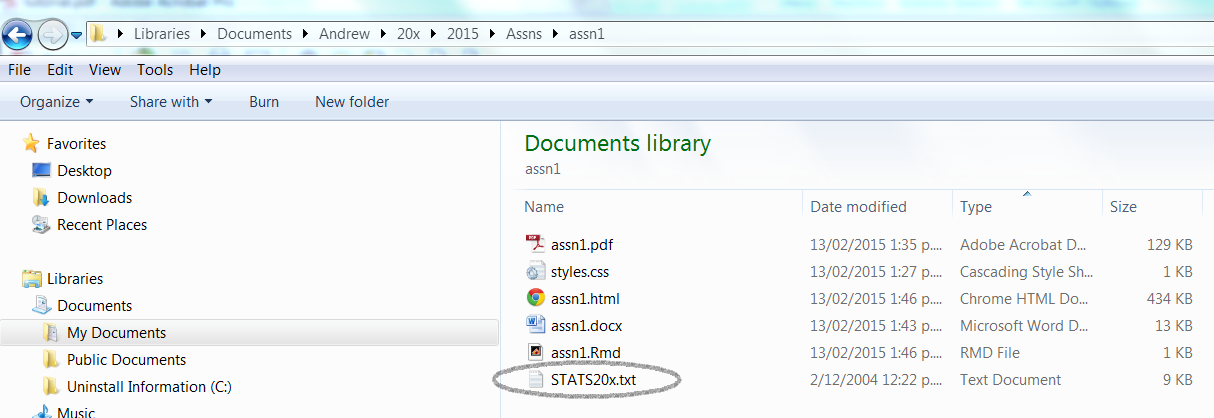
\includegraphics[width=4in]{Pictures/WhereData}
\end{center}

Text files often have \texttt{.txt} appended to their name. The letters after the full stop in the file name are sometimes called a file-name \emph{extension}, and are often used by the operating system (Windows, Mac OS X, Linux) to decide which application/programme should be used to open the file.

\end{frame}


\begin{frame}[fragile]
\frametitle{What do the data look like?}
As data analysts we love our data to be in `rectangular' (i.e., matrix or array) form.
Our raw data looks like this in the Notepad text editor.
\vspace{-3mm}
\begin{center}
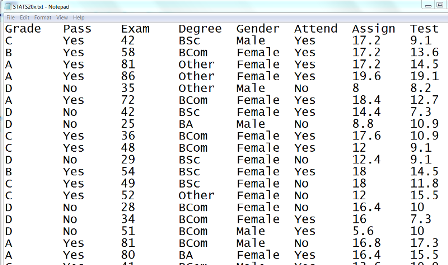
\includegraphics{Pictures/Stats20xdata}
\end{center}
\vspace{-3mm}
Note that the first row of this \rcode{.txt} file contains the variable (i.e. column) names.
Each row represents a different student. The columns within each row are separated by a  \rcode{TAB} character -- i.e. the file is  \emph{\rcode{TAB} delimited}.

\end{frame}


\begin{frame}[fragile]
\frametitle{How do we import this data-file?}
\begin{knitrout}\scriptsize
\definecolor{shadecolor}{rgb}{0.969, 0.969, 0.969}\color{fgcolor}\begin{kframe}
\begin{alltt}
\hlstd{> }\hlcom{## Importing data into R}
\hlstd{> }\hlstd{Stats20x.df} \hlkwb{=} \hlkwd{read.table}\hlstd{(}\hlstr{"Data/STATS20x.txt"}\hlstd{,} \hlkwc{header}\hlstd{=}\hlnum{TRUE}\hlstd{)}
\end{alltt}
\end{kframe}
\end{knitrout}
Here we are importing the \rcode{STATS20x.txt} data from a folder called \rcode{Data} that resides within our ``working directory''.
We are also telling \rcode{R} that the 1\textsuperscript{st} line of data contains the variable names by using
the argument \rcode{header = TRUE}.\footnote{\rcode{T} can be used as an abbreviation for \rcode{TRUE}. } \\[9mm]

If the data file resides in the working directory then it is enough to use
\begin{knitrout}\scriptsize
\definecolor{shadecolor}{rgb}{0.969, 0.969, 0.969}\color{fgcolor}\begin{kframe}
\begin{alltt}
\hlstd{> }\hlstd{Stats20x.df} \hlkwb{=} \hlkwd{read.table}\hlstd{(}\hlstr{"STATS20x.txt"}\hlstd{,} \hlkwc{header}\hlstd{=}\hlnum{TRUE}\hlstd{)}
\end{alltt}
\end{kframe}
\end{knitrout}

You can set the working directory using the \rcode{Session} menu of RStudio.

{\bf Note:} In \rcode{R} code, we preface comment lines with the  {\color{darkgreen}\verb|#|} symbol.

\end{frame}


%%%%%%%%%%%%%%%%%%%%%%%%%%%%%%%%%%%%%%%%%%%%%%%%%%%%%%%%%%%%%%%%%%%%%%%%%%%%%%%%%%%%%%%%%%%
\BeginSection{Working with dataframes in \rcode{R}}
%%%%%%%%%%%%%%%%%%%%%%%%%%%%%%%%%%%%%%%%%%%%%%%%%%%%%%%%%%%%%%%%%%%%%%%%%%%%%%%%%%%%%%%%%%%

\begin{frame}[fragile]
\frametitle{Where are the data?}

It is there all right!\footnote{Provided that you have {\bf Run} the code chunk -- knitting does not save the objects created.} 
The data exist in the \rcode{R} session as a dataframe object with the name \rcode{Stats20x.df}. 

You can use whatever name you want (within reason) for objects you create in your \rcode{R} session, so always try to use meaningful names that will help you remember what the object is. That is why we used the \rcode{.df} suffix for our dataframe.

To see the dataframe you just need to ask. For example:
\begin{knitrout}\scriptsize
\definecolor{shadecolor}{rgb}{0.969, 0.969, 0.969}\color{fgcolor}\begin{kframe}
\begin{alltt}
\hlstd{> }\hlcom{## 1st 5 rows and 7 columns of data set Stats20x.df}
\hlstd{> }\hlstd{Stats20x.df[}\hlnum{1}\hlopt{:}\hlnum{5}\hlstd{,}\hlnum{1}\hlopt{:}\hlnum{7}\hlstd{]}
\end{alltt}
\begin{verbatim}
  Grade Pass Exam Degree Gender Attend Assign
1     C  Yes   42    BSc   Male    Yes   17.2
2     B  Yes   58   BCom Female    Yes   17.2
3     A  Yes   81  Other Female    Yes   17.2
4     A  Yes   86  Other Female    Yes   19.6
5     D   No   35  Other   Male     No    8.0
\end{verbatim}
\end{kframe}
\end{knitrout}

\end{frame}


\begin{frame}[fragile]
\frametitle{How do we obtain the dimensions of a dataframe?}

What are the dimensions of the \rcode{Stats20x.df} dataframe?
\begin{knitrout}\scriptsize
\definecolor{shadecolor}{rgb}{0.969, 0.969, 0.969}\color{fgcolor}\begin{kframe}
\begin{alltt}
\hlstd{> }\hlkwd{dim}\hlstd{(Stats20x.df)}
\end{alltt}
\begin{verbatim}
[1] 146  15
\end{verbatim}
\end{kframe}
\end{knitrout}
It consists of 146 rows (students) and 15 columns. Each column represents a recorded measurement, characteristic, or feature of the students -- that is, a variable.

\medskip
{\bf Note:} {\rcode R} is case sensitive. For example, the dataframe \rcode{stats20x.df} does not exist, and so asking for its dimensions will give an error:

\begin{knitrout}\scriptsize
\definecolor{shadecolor}{rgb}{0.969, 0.969, 0.969}\color{fgcolor}\begin{kframe}
\begin{alltt}
\hlstd{> }\hlkwd{dim}\hlstd{(stats20x.df)}
\end{alltt}
\end{kframe}
\end{knitrout}

\begin{knitrout}\scriptsize
\definecolor{shadecolor}{rgb}{0.969, 0.969, 0.969}\color{fgcolor}\begin{kframe}
\begin{verbatim}
Error in try(dim(stats20x.df)) : object 'stats20x.df' not found
\end{verbatim}
\end{kframe}
\end{knitrout}

\end{frame}


\begin{frame}[fragile]
\frametitle{Summarising STATS 20x exam marks}
You can ask for one variable at a time using the \rcode{\$} sign after the dataframe name.
For example, we type \rcode{Stats20x.df\$Exam} to obtain the \rcode{Exam} variable.

Here we just look at the first 10 observations for brevity.
\begin{knitrout}\scriptsize
\definecolor{shadecolor}{rgb}{0.969, 0.969, 0.969}\color{fgcolor}\begin{kframe}
\begin{alltt}
\hlstd{> }\hlstd{Stats20x.df}\hlopt{$}\hlstd{Exam[}\hlnum{1}\hlopt{:}\hlnum{10}\hlstd{]}
\end{alltt}
\begin{verbatim}
 [1] 42 58 81 86 35 72 42 25 36 48
\end{verbatim}
\end{kframe}
\end{knitrout}

If we want to look at the distribution of \rcode{Exam}, the visualisation tool of choice will be a histogram. 

\end{frame}


\begin{frame}[fragile]
\frametitle{Summarising STATS 20x exam marks\ldots}
\framesubtitle{A histogram}
\medskip
\begin{knitrout}\scriptsize
\definecolor{shadecolor}{rgb}{0.969, 0.969, 0.969}\color{fgcolor}\begin{kframe}
\begin{alltt}
\hlstd{> }\hlcom{#Using xlab="STATS 20x exam score" to label the x-axis.}
\hlstd{> }\hlkwd{hist}\hlstd{(Stats20x.df}\hlopt{$}\hlstd{Exam,} \hlkwc{xlab}\hlstd{=}\hlstr{"STATS 20x exam score"}\hlstd{)}
\end{alltt}
\end{kframe}
\end{knitrout}



\begin{figure}
  \centering
  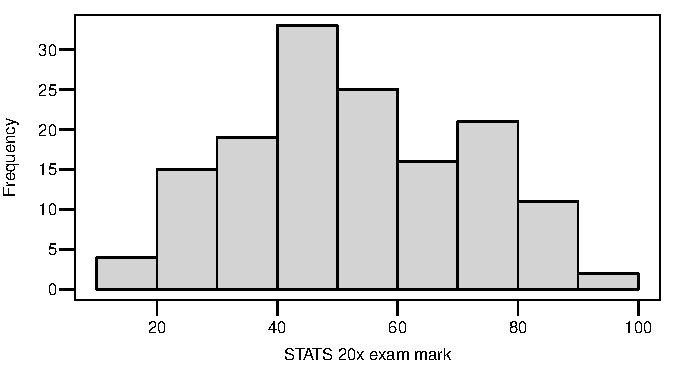
\includegraphics{figure/RC-H01-007}
\end{figure}

\end{frame}


\begin{frame}[fragile]
\frametitle{Summarising STATS 20x exam marks\ldots}
\framesubtitle{Numerical summaries}

Let us obtain some numerical summaries.

\begin{knitrout}\scriptsize
\definecolor{shadecolor}{rgb}{0.969, 0.969, 0.969}\color{fgcolor}\begin{kframe}
\begin{alltt}
\hlstd{> }\hlkwd{summary}\hlstd{(Stats20x.df}\hlopt{$}\hlstd{Exam)}
\end{alltt}
\begin{verbatim}
   Min. 1st Qu.  Median    Mean 3rd Qu.    Max. 
  11.00   40.00   51.50   52.88   68.50   93.00 
\end{verbatim}
\end{kframe}
\end{knitrout}
\begin{itemize}
\item So the lowest mark was 11 (\rcode{Min.}\,$\equiv$ minimum),
\item the highest 93 (\rcode {Max.}\,$\equiv$ maximum),
\item $\frac{1}{4}$ got 40 or less (\rcode{1st Qu.}\,$\equiv$ lower quartile),
\item $\frac{1}{2}$ got less/more than 51.5 (\rcode{Med.}\,$\equiv$  median),
\item $\frac{1}{4}$ got more than 68.5 (\rcode{3rd Qu.}\,$\equiv$ upper quartile),
\item and the average (\rcode{Mean}) mark was about 53 (52.88) marks.
\end{itemize}
%There may be evidence of two underlying populations? Discuss (or not).

\end{frame}



%%%%%%%%%%%%%%%%%%%%%%%%%%%%%%%%%%%%%%%%%%%%%%%%%%%%%%%%%%%%%%%%%%%%%%%%%%%%%%%%%%%%%%%%%%%
\BeginSection{How to  fit straight lines to your data - a.k.a. the simple linear model}
%%%%%%%%%%%%%%%%%%%%%%%%%%%%%%%%%%%%%%%%%%%%%%%%%%%%%%%%%%%%%%%%%%%%%%%%%%%%%%%%%%%%%%%%%%%


\begin{frame}
\frametitle{Example -- Former STATS 20x students' exam marks}
From the above summary we have some understanding about STATS 20x students' final exam marks. This is mildly interesting, but perhaps we could ask more interesting questions than this?

\medskip
\textbf{Here is one:}
\medskip
Does my mid-term test mark relate to my final exam mark?

\medskip
To be honest, I am pretty sure we know the answer to this question but let us answer this question, based on our data (not based on a strong opinion) and see if this suspected relationship is real or not.

\medskip
The specific research question addressed in this chapter is
{\bf can we use mid-term test score to explain final exam score?}
\end{frame}


\begin{frame}[fragile]
\frametitle{Exam vs.\ Test marks}
\framesubtitle{The particular variables of interest}

\begin{tabular}{lp{15cm}}
\rcode{Exam} &  the student's exam mark (out of 100) \\

\rcode{Test} & the student's Test mark (out of 20)\\

\end{tabular}

As scientists our first task is to determine whether or not there really is an association between \rcode{Test} and \rcode{Exam}.

If \rcode{Test} {\bf is} found to be associated with \rcode{Exam} then the next step is to quantify the magnitude of that relationship.
\medskip

{\bf Note:} that our question really is about the `typical' or average relationship.
Some students may do well in the term test but not in the exam and vice-versa.
We are really interested in the `expected' effect of test on exam.

\medskip
As our variables \rcode{Test} and \rcode{Exam} are both numerical we draw a scatter-plot to see what relationship is suggested (if any).
A scatter-plot (sometimes called a {\it xy}-plot) has two axes,
a horizontal {\it x}-axis and a vertical {\it y}-axis.

\end{frame}


\begin{frame}[fragile]
\frametitle{Exam vs.\ Test marks\ldots}
\framesubtitle{Let us look at these data}
\rcode{Test} is the explanatory (or independent) variable and goes on the {\it x}-axis.\\
\rcode{Exam} is the response (or dependent) variable and goes on the {\it y}-axis. \\
\phantom{A space}

\begin{knitrout}\scriptsize
\definecolor{shadecolor}{rgb}{0.969, 0.969, 0.969}\color{fgcolor}\begin{kframe}
\begin{alltt}
\hlstd{> }\hlcom{## Importing data into R}
\hlstd{> }\hlstd{Stats20x.df} \hlkwb{=} \hlkwd{read.table}\hlstd{(}\hlstr{"Data/STATS20x.txt"}\hlstd{,} \hlkwc{header}\hlstd{=T)}
\hlstd{> }\hlcom{## Plot the data}
\hlstd{> }\hlkwd{plot}\hlstd{(Exam} \hlopt{~} \hlstd{Test,} \hlkwc{data} \hlstd{= Stats20x.df)}
\end{alltt}
\end{kframe}
\end{knitrout}
\end{frame}


\begin{frame}[fragile]
\frametitle{Exam vs.\ Test marks\ldots}
\framesubtitle{Let us look at these data\ldots}



\begin{figure}
  \centering
  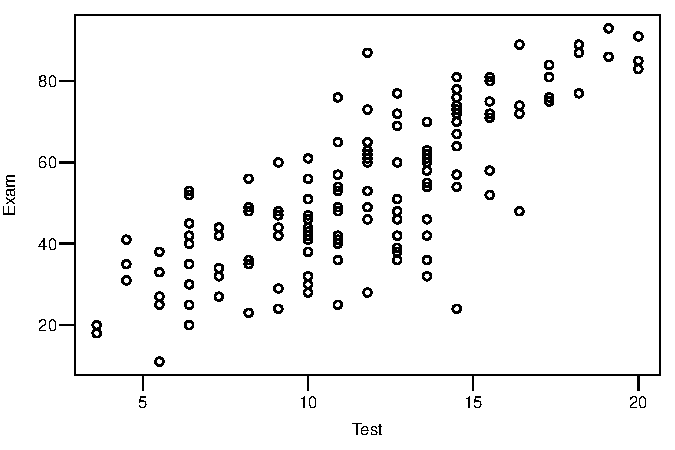
\includegraphics{figure/RC-H01-010}
\end{figure}

\end{frame}


\begin{frame}[fragile]
\frametitle{Exam vs.\ Test marks\ldots}
\framesubtitle{Let us look at these data\ldots}

{\bf Note} that the \rcode{plot(Exam \textasciitilde{} Test, data = Stats20x.df)} statement
asks \rcode{R} to produce a plot suitable for showing how  \rcode{Test} ({\it x}-axis variable)
is related to \rcode{Exam} ({\it y}-axis variable).

Looking at this plot, it is clear that there is some relationship,
but there is also a lot of variability in exam score amongst students with the same
test score, especially in the middle of the data.

\medskip As we are interested in the `typical' exam score 
for a given test score we would like to visually see
what the underlying trend is,
and how much the exam scores vary (scatter) about that trend.
It is helpful to run a smooth trend line through the scatter-plot.

\end{frame}


\begin{frame}[fragile]
\frametitle{Exam vs.\ Test marks\ldots}
\framesubtitle{Let us look at these data\ldots}

\begin{knitrout}\scriptsize
\definecolor{shadecolor}{rgb}{0.969, 0.969, 0.969}\color{fgcolor}\begin{kframe}
\begin{alltt}
\hlstd{> }\hlcom{## Load the s20x library to use the trendscatter function}
\hlstd{> }\hlkwd{library}\hlstd{(s20x)}
\hlstd{> }\hlkwd{trendscatter}\hlstd{(Exam} \hlopt{~} \hlstd{Test,} \hlkwc{data} \hlstd{= Stats20x.df)}
\end{alltt}
\end{kframe}
\end{knitrout}



\begin{figure}
  \centering
  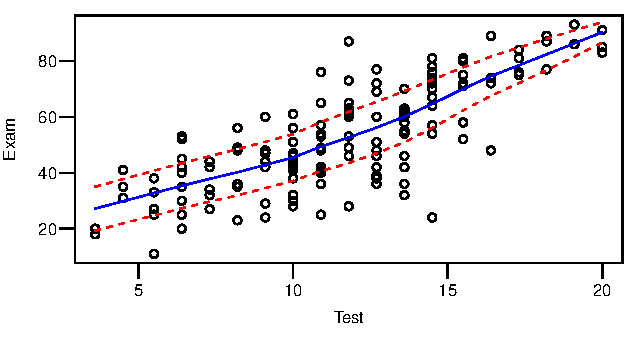
\includegraphics{figure/RC-H01-012}
\end{figure}

\end{frame}


\begin{frame}[fragile]
\frametitle{Exam vs.\ Test marks\ldots}
\framesubtitle{Let us look at these data\ldots}
This is our first application of a `bespoke'\footnote{(Of a computer program) written or adapted for a specific user or purpose: \it{``completely bespoke software systems''}  -- Oxford Dictionary.}
function, \rcode{trendscatter}, made just for you.
It is one of the many functions to be found when you load the \rcode {s20x} package.
The \rcode{trendscatter} function computes a lowess\footnote{\emph{lowess} stands for \underline{l}ocally \underline{w}eighted \underline{s}catterplot \underline{s}moothing.} smoother to the data (the {\color{blue} blue} line) along with estimates of the variation about that line (the {\color{red}red} lines).

\medskip The underlying trend here looks like a straight line.
The variability looks roughly constant -- except, perhaps,
for those students who got high test marks.

{\bf Note:} When we talk about ``variability'' it is in the vertical direction.
That is, we are talking about the variability in exam score for a given fixed value
of test score.

\end{frame}



%%%%%%%%%%%%%%%%%%%%%%%%%%%%%%%%%%%%%%%%%%%%%%%%%%%%%%%%%%%%%%%%%%%%%%%%%%%%%%%%%%%%%%%%%%%
\BeginSection{How to predict using the fitted model?}
%%%%%%%%%%%%%%%%%%%%%%%%%%%%%%%%%%%%%%%%%%%%%%%%%%%%%%%%%%%%%%%%%%%%%%%%%%%%%%%%%%%%%%%%%%%


\begin{frame}[fragile]
\frametitle{Exam vs.\ Test marks\ldots}
\framesubtitle{Fitting a simple linear model}
\begin{large}\centering
\textbf{Pro Tip:} If it looks like a straight line then fit a straight line.\\
\end{large}
\vspace{12pt}
A straight line is a simple (but not the simplest) form  of a linear model.

\medskip
\begin{knitrout}\scriptsize
\definecolor{shadecolor}{rgb}{0.969, 0.969, 0.969}\color{fgcolor}\begin{kframe}
\begin{alltt}
\hlstd{> }\hlstd{examtest.fit} \hlkwb{=} \hlkwd{lm}\hlstd{(Exam} \hlopt{~} \hlstd{Test,} \hlkwc{data} \hlstd{= Stats20x.df)}
\hlstd{> }\hlkwd{summary}\hlstd{(examtest.fit)}
\end{alltt}
\end{kframe}
\end{knitrout}

\begin{knitrout}\scriptsize
\definecolor{shadecolor}{rgb}{0.969, 0.969, 0.969}\color{fgcolor}\begin{kframe}
\begin{verbatim}
Coefficients:
            Estimate Std. Error t value Pr(>|t|)    
(Intercept)   9.0845     3.2204   2.821  0.00547 ** 
Test          3.7859     0.2647  14.301  < 2e-16 ***
---
Residual standard error: 12.05 on 144 degrees of freedom
Multiple R-squared:  0.5868,	Adjusted R-squared:  0.5839 
F-statistic: 204.5 on 1 and 144 DF,  p-value: < 2.2e-16
\end{verbatim}
\end{kframe}
\end{knitrout}

Note that \rcode{examtest.fit} now resides in our \rcode{R} session as an \rcode{lm} \emph{object}. An object, in the \rcode{R} language, is a structure than can contain data, variables, functions or other objects.

\end{frame}



\begin{frame}[fragile]
\frametitle{Exam vs.\ Test marks\ldots}
\framesubtitle{The simple linear model}
Let us see what this means.\\
\vspace{12pt}

The summary output has a number of different components.
Let us start with the \rcode{Estimate} column.

You will (or should!) recall from high school and/or STATS 10x that the equation for a straight line,
\[
y=a+bx,
\]
is described using two numbers (parameters), where:\\
\begin{itemize}
\item $a$ is called the \emph{intercept} since it is the value of $y$ when the line intercepts the y-axis. Note that the y-axis corresponds to $x=0$.

\item $b$ is called the \emph{slope}. It tells us the rate of increase (or decrease) in $y$, for every additional unit increase in the value $x$.
\end{itemize}

\end{frame}



\begin{frame}[fragile]
\frametitle{Exam vs.\ Test marks\ldots}
\framesubtitle{The simple linear model}
In the linear modelling context,
it is the expected value of variable $y$, $\E[Y|x]$,
that is assumed to follow a linear relationship with $x$. We read $\E[Y|x]$ as ``the expected value of $y$ given $x$.'' This is called a \emph{conditional expectation}. It means that the expected value (or mean) of $y$ will, or may, change depending on the value of $x$.
That is, we assume
\[
\E[Y|x]=a+bx
\]

The first row of the above \rcode{summary(examtest.fit)} table is labelled \rcode{Intercept}, and in the \rcode{Estimate} column is the estimated value
of $a$ (i.e., the estimated value of $y=$ \rcode{Exam} when $x=$ \rcode{Test = 0}). 
The second row gives the estimated value of $b$, which is the increase in expected value of $y=$ \rcode{Exam} when $x=$ \rcode{Test} increases by one mark.

\end{frame}


\begin{frame}[fragile]
\frametitle{Exam vs.\ Test marks\ldots}
\framesubtitle{The simple linear model, general notation}

In the previous slides we used $a$ and $b$ to denote the intercept and slope parameters. 
This is just a naming choice, and we could have used 
\[
\E[Y|x]=\theta+\gamma x
\] or
\[
\E[Y|x]=c+dx,
\] or
\[
\E[Y|x]=\beta_0+\beta_{1}x \ .
\]

In this class we shall use the $\beta_0$, $\beta_1$, choice of parameter names
since it is easiest to generalize to more complex models having many parameters.

\end{frame}




\begin{frame}[fragile]
\frametitle{Exam vs.\ Test marks\ldots}
\framesubtitle{The simple linear model}
In the linear modelling context,
it is the expected or typical value of variable $y$ that follows a linear model. 
So, for the simple linear model:
\[
\E[Y|x]=\beta_0+\beta_{1}x.
\]
We can say that each $y$ can be broken into what we expect to see plus a component that is random and, therefore, cannot be explained.\footnote{This also applies to the more complex linear models we see later.}

We can write this as
\[
y=\E[Y|x]+\varepsilon=\beta_0+\beta_{1}x+\varepsilon
\]
where $\varepsilon$ (epsilon) is random with expected value 0. This expresses how an observation varies around its expected or typical value. We will discuss these ideas  in greater detail in the next chapter.

\end{frame}


\begin{frame}[fragile]
\frametitle{Exam vs.\ Test marks\ldots}
\framesubtitle{Let us look at this model}

Let us extract the coefficients component from the fitted model object:

\begin{knitrout}\scriptsize
\definecolor{shadecolor}{rgb}{0.969, 0.969, 0.969}\color{fgcolor}\begin{kframe}
\begin{alltt}
\hlstd{> }\hlkwd{coef}\hlstd{(examtest.fit)}
\end{alltt}
\begin{verbatim}
(Intercept)        Test 
   9.084463    3.785924 
\end{verbatim}
\end{kframe}
\end{knitrout}



You can see this corresponds to the \rcode{Estimate} column of the regression summary table.

We are saying that the `best' fit of the data tells us that the predicted exam score
for a student with test score \rcode{Test} is given by the
following equation (to two decimal places):
\begin{center}
$ \widehat{\rcode{Exam}}=9.08+3.79\times \rcode{Test}$\footnote{ We use the notation $\widehat{\rcode{Exam}}$ as this is an estimated value.}.
\end{center}

\end{frame}


\begin{frame}[fragile]
\frametitle{Exam vs.\ Test marks\ldots}
\framesubtitle{Let us look at this model\ldots}
So, if you have received $0$ in the \rcode{Test}, then we estimate that you should be able (on average) to get 9.08 marks for just turning up to the exam and guessing your way through it.

\medskip

Thereafter, for every extra mark you get in the the test (out of 20) your final exam score will increase (on average) by about 3.79 marks.

\medskip

Here are some predictions for typical students who got test mark of 0, 10 or 20:
\begin{itemize}
\item \rcode{Test = \phantom{0}0} then $\widehat{\rcode{Exam}}=9.08+3.79\times \phantom{0}0 =\phantom{0}9.08\%$ in the exam,

\item \rcode{Test = 10} then $\widehat{\rcode{Exam}}=9.08+3.79\times 10 =46.94\%$ in the exam,

\item \rcode{Test = 20} then $\widehat{\rcode{Exam}}=9.08+3.79\times 20 =84.80\%$ in the exam.
\end {itemize}

\end{frame}


\begin{frame}[fragile]
\frametitle{Exam vs.\ Test marks\ldots}
\framesubtitle{Let us look at this model\ldots}
Let us see how this model works out overall.
Here we are plotting the `best' estimated straight line that we obtained from fitting our model. \\
\phantom{A space}

\begin{knitrout}\scriptsize
\definecolor{shadecolor}{rgb}{0.969, 0.969, 0.969}\color{fgcolor}\begin{kframe}
\begin{alltt}
\hlstd{> }\hlkwd{plot}\hlstd{(Exam} \hlopt{~} \hlstd{Test,} \hlkwc{data} \hlstd{= Stats20x.df,} \hlkwc{xlim} \hlstd{=} \hlkwd{c}\hlstd{(}\hlnum{0}\hlstd{,} \hlnum{20}\hlstd{))}
\hlstd{> }\hlcom{## Add the lm estimated line to this plot}
\hlstd{> }\hlkwd{abline}\hlstd{(examtest.fit,} \hlkwc{lty} \hlstd{=} \hlnum{2}\hlstd{,} \hlkwc{col} \hlstd{=} \hlstr{"blue"}\hlstd{)}
\hlstd{> }\hlcom{## Calculate predicted values for students who get test=0,10,20}
\hlstd{> }\hlstd{predns}\hlkwb{=}\hlkwd{predict}\hlstd{(examtest.fit,} \hlkwc{newdata} \hlstd{=} \hlkwd{data.frame}\hlstd{(}\hlkwc{Test}\hlstd{=}\hlkwd{c}\hlstd{(}\hlnum{0}\hlstd{,}\hlnum{10}\hlstd{,}\hlnum{20}\hlstd{)))}
\hlstd{> }\hlcom{## Add the predicted values to the plot}
\hlstd{> }\hlkwd{points}\hlstd{(}\hlkwd{c}\hlstd{(}\hlnum{0}\hlstd{,}\hlnum{10}\hlstd{,}\hlnum{20}\hlstd{), predns,}\hlkwc{col} \hlstd{=} \hlstr{"blue"}\hlstd{,} \hlkwc{pch} \hlstd{=} \hlnum{19}\hlstd{)}
\end{alltt}
\end{kframe}
\end{knitrout}

\end{frame}


\begin{frame}[fragile]
\frametitle{Exam vs.\ Test marks\ldots}
\framesubtitle{Let us look at this model\ldots}



\begin{figure}
  \centering
  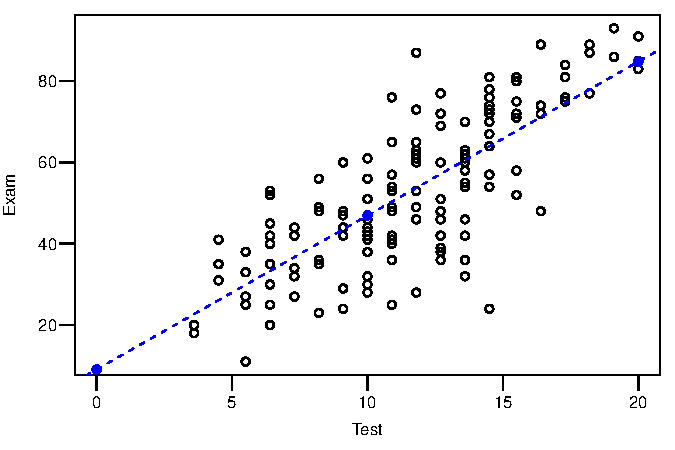
\includegraphics{figure/RC-H01-019}
\end{figure}

\end{frame}


%%%%%%%%%%%%%%%%%%%%%%%%%%%%%%%%%%%%%%%%%%%%%%%%%%%%%%%%%%%%%%%%%%%%%%%%%%%%%%%%%%%%%%%%%%%
\BeginSection{How good is the fitted model for prediction?  --  $R^2$}
%%%%%%%%%%%%%%%%%%%%%%%%%%%%%%%%%%%%%%%%%%%%%%%%%%%%%%%%%%%%%%%%%%%%%%%%%%%%%%%%%%%%%%%%%%%


\begin{frame}[fragile]
\frametitle{Exam vs.\ Test marks\ldots}
\framesubtitle{The null model}
This model is not too bad. It appears to do a reasonable job of describing the data and appears to make sense -- but compared to what? How useful is the variable  \rcode{Test} in explaining and predicting \rcode{Exam}?

We can fit a model that is even simpler than the straight line model. This is called the null\footnote{The null model is the model assumed by a one sample \ttest{}, as seen in Chapter 3.} model and simply estimates the  typical exam mark without an explanatory variable $x$. That is , $\E[Y|x]=\E[Y]$. Here is our null model for $y=Exam$: 
\vspace{-0.5em}
\begin{align*}
y &=\E[Y|x]+\varepsilon\\
  &=\E[Y] +\varepsilon\\
  &=\beta_0+\varepsilon\\
  &\equiv \mu+\varepsilon
\end{align*}
That is, $x=Test$, say, is not related to exam mark.

\end{frame}


\begin{frame}[fragile]
\frametitle{Exam vs.\ Test marks\ldots}
\framesubtitle{The null model\ldots}
Let us fit this $null$ model:
\begin{knitrout}\scriptsize
\definecolor{shadecolor}{rgb}{0.969, 0.969, 0.969}\color{fgcolor}\begin{kframe}
\begin{alltt}
\hlstd{> }\hlcom{## Null model}
\hlstd{> }\hlstd{examnull.fit}\hlkwb{=}\hlkwd{lm}\hlstd{(Exam} \hlopt{~} \hlnum{1}\hlstd{,} \hlkwc{data} \hlstd{= Stats20x.df)}
\hlstd{> }\hlkwd{summary}\hlstd{(examnull.fit)}
\end{alltt}
\end{kframe}
\end{knitrout}
\begin{knitrout}\scriptsize
\definecolor{shadecolor}{rgb}{0.969, 0.969, 0.969}\color{fgcolor}\begin{kframe}
\begin{verbatim}
Coefficients:
            Estimate Std. Error t value Pr(>|t|)    
(Intercept)   52.877      1.546   34.21   <2e-16 ***
---
Residual standard error: 18.68 on 145 degrees of freedom
\end{verbatim}
\end{kframe}
\end{knitrout}

In comparison, the simple linear model \rcode{examtest.fit}
gives us different predictions for different test marks. Naturally we would suspect this to be a better model for predicting $Exam$ as we are pretty sure that $Test$ explains $Exam$ quite well.

\end{frame}


\begin{frame}[fragile]
\frametitle{Exam vs.\ Test marks\ldots}
\framesubtitle{The null model\ldots}
Our null model was $Exam =\beta_0 +\varepsilon$ where $\varepsilon \iid N(0, \sigma_{Null}^2)$\footnote {If we were were doing a one sample \ttest{} we would use parameter name $\mu$ instead of the more general $\beta_0$.} with the best estimate of $\mu=\beta_0$ being the
sample mean, $\bar{y}=52.88$.

\medskip
Note that the estimate of the standard deviation ($\sigma$) of the random $\varepsilon$ component  was $\hat{\sigma}_{Null}=s_{Null}=18.68$.\footnote{Here we use the hat notation to denote that $\hat{\sigma}_{Null}$ is an estimate of the unknown parameter $\sigma_{Null}$. }

This is also called the residual standard error.

\end{frame}




\begin{frame}[fragile]
\frametitle{Exam vs.\ Test marks\ldots}
\framesubtitle{Null vs. simple linear model}

Compare the null model to the simple linear model that
used \rcode{Test} as an explanatory variable.
\begin{knitrout}\scriptsize
\definecolor{shadecolor}{rgb}{0.969, 0.969, 0.969}\color{fgcolor}\begin{kframe}
\begin{alltt}
\hlstd{> }\hlcom{## Exam vs. Test model}
\hlstd{> }\hlkwd{summary}\hlstd{(examtest.fit)}
\end{alltt}
\end{kframe}
\end{knitrout}

\begin{knitrout}\scriptsize
\definecolor{shadecolor}{rgb}{0.969, 0.969, 0.969}\color{fgcolor}\begin{kframe}
\begin{verbatim}
Coefficients:
            Estimate Std. Error t value Pr(>|t|)    
(Intercept)   9.0845     3.2204   2.821  0.00547 ** 
Test          3.7859     0.2647  14.301  < 2e-16 ***
---
Residual standard error: 12.05 on 144 degrees of freedom
Multiple R-squared:  0.5868,	Adjusted R-squared:  0.5839 
F-statistic: 204.5 on 1 and 144 DF,  p-value: < 2.2e-16
\end{verbatim}
\end{kframe}
\end{knitrout}

Note that the estimate $(s_{Test})$ of the standard deviation
$(\sigma_{Test})$ of the  random $(\varepsilon)$ component 
has been reduced to $s_{Test}=12.05$.

\end{frame}


\begin{frame}[fragile]
\frametitle{Exam vs.\ Test marks\ldots}
\framesubtitle{How good is this simple linear model?}

If $y=\rcode{Exam}$ and $x=\rcode{Test}$, then here are our fitted null (the {\color{red} red} line) and linear (the {\color{blue} blue} line) models. We clearly see that the blue line does a far better job of describing this relationship than the red line.  

% Null model: $y=\beta_0+\varepsilon$ (red) versus 
% $y=\beta_0+\beta_1 x+\varepsilon$ (blue) where $\varepsilon\iid N(0,\sigma^2)$:



\begin{figure}
  \centering
  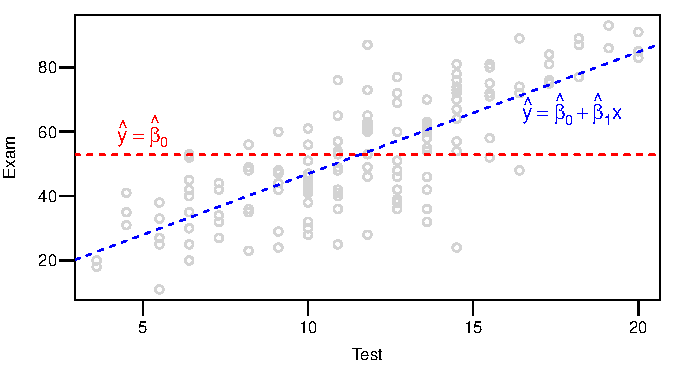
\includegraphics{figure/RC-H01-020A}
\end{figure}

\end{frame}


\begin{frame}[fragile]
\frametitle{Exam vs.\ Test marks\ldots}
\framesubtitle{Multiple R-squared}

The overall variation in the null model is given by the sum of the squared residuals, 
denoted by $SS_{Null}$.
In Chapter 2 we will see that $SS_{Null}=50586$.
$SS_{Null}$ is more commonly known as the {\bf total sum of squares}, $SS_{Tot}$.

The sum of squares of the residuals from the model using the variable \rcode{Test}, 
denoted here by $SS_{Test}$, is $20901$.

The reduction in overall variation from the \rcode{Null} model to the \rcode{Test} model can be expressed as a proportion of $SS_{Null}$:

\medskip 
\begin{center}
$\frac{SS_{Null} - SS_{Test}}{SS_{Null}}=1-\frac{SS_{Test}}{SS_{Null}} =1-\frac{20901}{50586}\approx 0.59.$
\end{center}

This statistic is usually called multiple {\bf R-squared} ($R^2$) or the proportion of variation explained.

\medskip
In the above output it is: \rcode{Multiple R-squared: 0.5868}
\end{frame}


\begin{frame}[fragile]
\frametitle{R-squared interpretation}

We can say that ($100\times R^2)= 59\%$ of the (total) variation in the exam mark is explained by using a straight line relationship (i.e., simple linear model) with
test score.

So by using just one explanatory variable, $x=Test$,  we can explain 59\% of the variation that we observe in $y=Exam$.
That is a pretty good return on one `piece of information', the \rcode{Test} score.
\medskip \medskip

You may have seen (from STATS 210 perhaps) that the estimates of 
$\sigma_{Null}$ and $\sigma_{Test}$ are obtained from the residual sums of squares:
$s_{Null}=\sqrt{SS_{Null}/(n-1)}$ and $s_{Test}=\sqrt{SS_{Test}/(n-2)}$.
\medskip

In the above calculation, $n$ is the number of observations ($n=146$ in this example), 
and $n-1$ is the degrees of freedom of the null model 
and $n-2$ is the degrees of freedom of the straight line model.

\end{frame}


\begin{frame}
\frametitle{Word of caution}

\medskip

In practice we need to first check the assumptions of our model before we can safely
use it for inference such as calculating confidence intervals, making predictions, etc.
\medskip

This is the focus of the next Chapter.
\end{frame}


%%%%%%%%%%%%%%%%%%%%%%%%%%%%%%%%%%%%%%%%%%%%%%%%%%%%%%%%%%%%%%%%%%%%%%%%%%%%%%%%%%%%%%%%
\BeginSection{Some technical asides}
%%%%%%%%%%%%%%%%%%%%%%%%%%%%%%%%%%%%%%%%%%%%%%%%%%%%%%%%%%%%%%%%%%%%%%%%%%%%%%%%%%%%%%%%

\begin{frame}[fragile]
\frametitle{Aside: Getting help on functions in R}

In this first chapter we have already used several \rcode{R} functions. It is easy to forget the details (e.g., the arguments that the function needs), in which case you can get help about the function by simply preceding its name with a question mark.

For example, try
\begin{knitrout}\scriptsize
\definecolor{shadecolor}{rgb}{0.969, 0.969, 0.969}\color{fgcolor}\begin{kframe}
\begin{alltt}
\hlstd{> }\hlopt{?}\hlstd{summary}
\end{alltt}
\end{kframe}
\end{knitrout}
\vspace{-0.5em}

or
\begin{knitrout}\scriptsize
\definecolor{shadecolor}{rgb}{0.969, 0.969, 0.969}\color{fgcolor}\begin{kframe}
\begin{alltt}
\hlstd{> }\hlopt{?}\hlstd{lm}
\end{alltt}
\end{kframe}
\end{knitrout}

In RStudio this opens a sub-window for the help file. It can be useful to look at the examples (at the bottom of the help file) of a function's usage to get an idea of how it is used.

Unfortunately, the \rcode{R} help can be rather difficult to understand at first because of all the computer jargon it uses. There is plenty of other online help on most \rcode{R} functions that can be found through your favourite search engine.

\end{frame}


\begin{frame}[fragile]
\frametitle{Aside: Data types in R}
There are several data types in \rcode{R}, but the three that we need to know about are \emph{numerical}, \emph{character} and \emph{logical}.
\bigskip

We'll see in Chapter 5 that we can also use character data as an explanatory variable. In that chapter we use the character variable class attendance ("Yes" or "No") to explain exam mark. We regard attendance as a two-level factor variable  --  stay tuned...

\begin{knitrout}\scriptsize
\definecolor{shadecolor}{rgb}{0.969, 0.969, 0.969}\color{fgcolor}\begin{kframe}
\begin{alltt}
\hlstd{> }\hlkwd{summary}\hlstd{(Stats20x.df}\hlopt{$}\hlstd{Attend)}
\end{alltt}
\begin{verbatim}
   Length     Class      Mode 
      146 character character 
\end{verbatim}
\end{kframe}
\end{knitrout}

\begin{knitrout}\scriptsize
\definecolor{shadecolor}{rgb}{0.969, 0.969, 0.969}\color{fgcolor}\begin{kframe}
\begin{alltt}
\hlstd{> }\hlkwd{summary}\hlstd{(}\hlkwd{as.factor}\hlstd{(Stats20x.df}\hlopt{$}\hlstd{Attend))}
\end{alltt}
\begin{verbatim}
 No Yes 
 46 100 
\end{verbatim}
\end{kframe}
\end{knitrout}

\end{frame}



%%%%%%%%%%%%%%%%%%%%%%%%%%%%%%%%%%%%%%%%%%%%%%%%%%%%%%%%%%%%%%%%%%%%%%%%%%%%%%%%%%%%%%%%%%%
\BeginSection{Relevant \rcode{R}-code}
%%%%%%%%%%%%%%%%%%%%%%%%%%%%%%%%%%%%%%%%%%%%%%%%%%%%%%%%%%%%%%%%%%%%%%%%%%%%%%%%%%%%%%%%%%%


\begin{frame}[fragile]
\frametitle{Most of the \rcode{R}-code you need for this chapter}


Creating a data frame by importing the text file \rcode{Data/STATS20x.txt} from the subfolder \rcode{Data}:

\begin{knitrout}\scriptsize
\definecolor{shadecolor}{rgb}{0.969, 0.969, 0.969}\color{fgcolor}\begin{kframe}
\begin{alltt}
\hlstd{> }\hlstd{Stats20x.df} \hlkwb{=} \hlkwd{read.table}\hlstd{(}\hlstr{"Data/STATS20x.txt"}\hlstd{,} \hlkwc{header}\hlstd{=}\hlnum{TRUE}\hlstd{)}
\end{alltt}
\end{kframe}
\end{knitrout}

Plotting a scatter plot of y (Exam) vs. x  (Test):

\begin{knitrout}\scriptsize
\definecolor{shadecolor}{rgb}{0.969, 0.969, 0.969}\color{fgcolor}\begin{kframe}
\begin{alltt}
\hlstd{> }\hlkwd{plot}\hlstd{(Exam}\hlopt{~}\hlstd{Test,} \hlkwc{data}\hlstd{=Stats20x.df)}
\end{alltt}
\end{kframe}
\end{knitrout}

and/or a trend-scatter-plot:

\begin{knitrout}\scriptsize
\definecolor{shadecolor}{rgb}{0.969, 0.969, 0.969}\color{fgcolor}\begin{kframe}
\begin{alltt}
\hlstd{> }\hlkwd{trendscatter}\hlstd{(Exam} \hlopt{~}\hlstd{Test,} \hlkwc{data} \hlstd{= Stats20x.df)}
\end{alltt}
\end{kframe}
\end{knitrout}


Fitting a linear (straight line) model and getting the estimated values:


\begin{knitrout}\scriptsize
\definecolor{shadecolor}{rgb}{0.969, 0.969, 0.969}\color{fgcolor}\begin{kframe}
\begin{alltt}
\hlstd{> }\hlstd{examtest.fit}\hlkwb{=}\hlkwd{lm}\hlstd{(Exam}\hlopt{~}\hlstd{Test,} \hlkwc{data}\hlstd{=Stats20x.df)}
\hlstd{> }\hlkwd{summary}\hlstd{(examtest.fit)}
\end{alltt}
\end{kframe}
\end{knitrout}

Adding your fitted/predicted blue-dashed line to the scatter-plot created above:

\begin{knitrout}\scriptsize
\definecolor{shadecolor}{rgb}{0.969, 0.969, 0.969}\color{fgcolor}\begin{kframe}
\begin{alltt}
\hlstd{> }\hlkwd{abline}\hlstd{(examtest.fit,} \hlkwc{lty} \hlstd{=} \hlnum{2}\hlstd{,} \hlkwc{col} \hlstd{=} \hlstr{"blue"}\hlstd{)}
\end{alltt}
\end{kframe}
\end{knitrout}

\end{frame}


\end{document}

%Notes modified Feb 2021 to no longer use random variable capitalization.
\begin{frame}
\frametitle{Aside: Notation}
You might have noticed that sometimes we use upper-case letters, and sometimes we use lower-case letters when talking about variables.

There is actually a meaning to the change in case. A convention in statistics is to write random variables in upper-case, and observed or fixed values in lower-case letters. When we write out the linear model we write
\[
y = \E[Y|x] + \varepsilon
\]
In this expression $X$ and $Y$ are random variables. When we write
\[
\beta_0 + \beta_1x + \varepsilon
\]
We are talking about the distribution of $Y$ for a particular value of $X$, i.e. $x$. If this does not mean much to you, or is incomprehensible, then do not worry about it. We just like you to know there is some logic here.

\end{frame}

